
% 1. Describe and explain the similarities and/or differences between the absorption, emission, and
% excitation spectra of Ru(bpy)32+∗. (Hint: Use Figure 2.)

% 2. Normalise the emission spectra to the maximum emission intensity for each Fe3+ and Cu2+ concen-
% tration in the luminescence quenching measurements. What happens to the shape of the spectra as the Fe3+ or Cu2+ concentration increases? Why? (Hint: Plot the absorption spectra of one of the Fe3+-containing samples and one of the Cu2+-containing samples and compare them to the
% absorption spectrum of the pure Rubpy2+ sample).

% 3. Compare the quenching rate coefficients obtained from the Stern–Volmer plots with the electron-
% transfer rate coefficients calculated from Marcus theory and comment on any similarities or differ-
% ences. Note that the rate coefficient for diffusion-controlled collisions between electron-transfer
% partners under the conditions studied is ∼3.3 × 109 M−1 s−1.

% 4. Compare the rate coefficients for Fe3+ and Cu2+ (both experimental and calculated) and explain the
% similarities or differences.
\textbf{Question 1}
As shown in Figure \ref{fig:part1_noq}, the absorption and excitation spectra of \ce{Rub(bpy)_{3}^{2+}} are essentially the same due to fluorescence occurring as the molecule returns to the electronic ground state following absorption. The excitation spectrum shows the relative intensity of fluorescence in relation to wavelength, whereas the absorption spectrum shows the relative intensity of light absorbed in relation to wavelength. Thus, the relative intensity and wavelengths at which these processes occur will match.
The emission spectrum shows relative intensity at which wavelengths of light are emitted (ie NOT absorbed) by a sample, and as such does not match excitation or absorption spectra. 

\noindent \textbf{Question 2}
Figure \ref{fig:part1_dis_q2} shows that the  
\begin{figure}[H]
     \centering
     \begin{subfigure}[b]{0.49\textwidth}
         \centering
         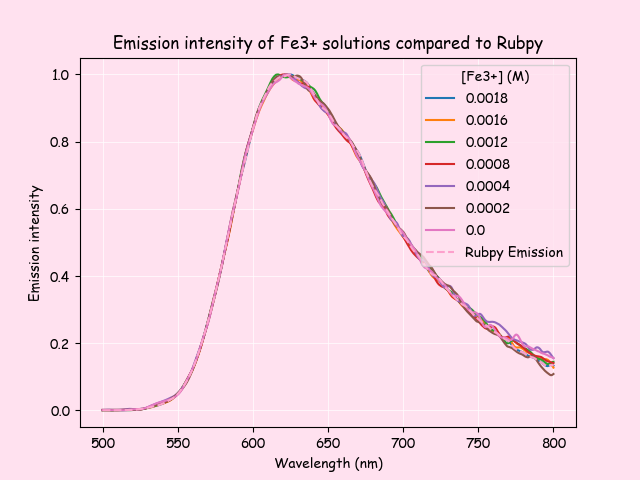
\includegraphics[width=\textwidth]{part1_discussionq2_fe.png}
         \caption{\ce{Fe^{3+}}}
         \label{fig:part1_dis_fe}
     \end{subfigure}
     \hfill
     \begin{subfigure}[b]{0.49\textwidth}
         \centering
         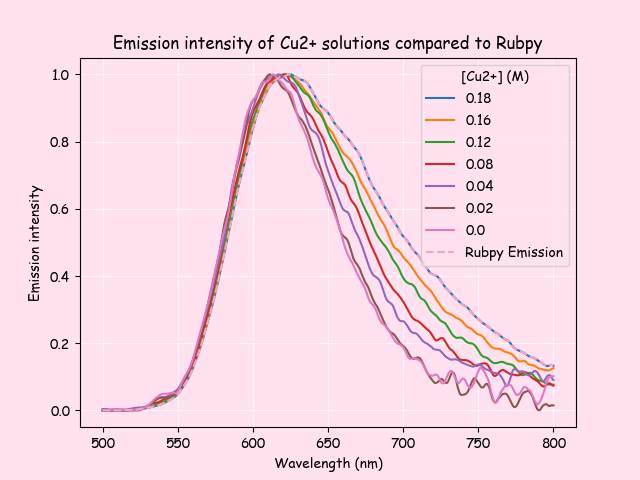
\includegraphics[width=\textwidth]{part1_discussionq2_cu.png}
         \caption{\ce{Cu^{2+}}}
         \label{fig:part1_dis_Cu}
     \end{subfigure}
     \caption{Normalised emission spectra for each concentration in the luminescence quenching measurements.}
     \label{fig:part1_dis_q2}
\end{figure}
